\documentclass[output=paper]{langscibook} 
\author{Bertille Baron\affiliation{Georgetown University}}
\title{DP-internal Structure and Agreement in Nafara}

% \chapterDOI{} %will be filled in at production
 
\abstract{Senufo Nafara DPs show the particularly rare unmarked word order [N AP Def Dem Numeral]. In this cartographic account, the proposed derivation uses spec-to-spec movement operations to generate this word order \citep{Cinque2005}. This analysis relies on two main claims: there is a domain ƩP under Num \citep{Aboh2004} in which two distinct categories of adjectives (high and low following \citealt{Cinque1994}) merge to modify the noun. It is this same ƩP domain that undergoes spec-to-spec movement, motivated for agreement purposes. Oppositely, all elements structurally above ƩP remain in situ.
}
\maketitle

\begin{document}
  

\section{Introduction}

Nafara is a Senufo language\footnote{Although there is some controversy over its classification (\citealt{Manessy1975,Naden1989}), Senufo is traditionally defined as a branch of the Niger-Congo, Gur subgroup (\citealt{Westermann1970}, \citealt{BendorSamuel1971}).} spoken in Korhogo, Côte d’Ivoire. Determiner phrases in the language show the canonical word order [N Adj D Dem Num], like in \REF{ex:baron:1} below. 


\ea
\glll lo  tã -gəl  gal kɔrʃi \label{ex:baron:1}\\
      mango sweet -\textsc{def.3.pl} \textsc{dem.3.pl} seven\\
      N Adj -D Dem Num\\
\glt \textit{‘these} \textit{seven} \textit{sweet} \textit{mangoes’}\footnote{The data introduced and analyzed throughout this paper was elicited from a native speaker of Senufo Nafara.}
\z

As we see here, attributive adjectives usually directly follow the noun. While they do not seem to show agreement, adjectives are apparently the host for the number and gender specific determiner.\footnote{The noun classification adopted in this paper is adapted from those provided by both \citet[22]{Manessy1996} and \citet[76]{Carlson1990} for other Senufo varieties. Nafara shows a 5-gender system, where genders 1, 2, and 3 consist of countable nouns, and genders 4 and 5 are for non-count nouns. Considering the scope of this paper, I will limit my discussion to countable nouns.} The demonstrative directly follows the determiner, and inflects for number and gender also. Numerals are DP-final in the language, and do not show concord.\footnote{This is true of all numerals except ‘one’ which shows gender agreement, as shown in \sectref{sec:baron:2.1.4}.}

The DP word order in \REF{ex:baron:1} is highly unexpected, as argued by \citet{Cinque2005}. First, cross-linguistically, Numerals in DP-final position are noticeably rare. Then, syntactically speaking, the derivation of this word order is usually considered marked \citep{Cinque2005}.

This paper accounts for both the syntactic structure and derivation of Nafara DPs, assuming the universal functional hierarchy [ Dem > Num > Adj > N ] adopted by \citet{Greenberg1963}, \citet{Cinque2005} and others. In \sectref{sec:baron:2.1}, I first discuss the location of each DP-internal element. I also draw distinctions between two separate categories of adjectives (that I refer to as high and low, corresponding to \citealt{Cinque2010}’s  indirect and direct modification respectively). In \sectref{sec:baron:2.2}, I motivate the movement of adjectives and noun only, responsible for the surface word order. Finally, in \sectref{sec:baron:2.3}, I show that such movement is motivated for agreement purposes.


\section{DP structure and word order} 
\subsection{Assumptions and data}
\label{sec:baron:2.1}
\subsubsection{The functional structure of DPs}
\label{sec:baron:2.1.1}
In a cartographic approach to DP structure, \citet{Greenberg1963} and \citet{Cinque2005} argue that the only possible initial order capable of universally generating the DP word orders attested in natural language is [ Dem > Num > Adj > N ]. Assuming the underlying structure in \figref{fig:baron:1}, Cinque accounts for all possible word orders as the result of some type of movement of NP. Namely, he argues for combinations of successive Spec-to-Spec movements with or without pied-piping of NP up the DP spine. 

  
\begin{figure} 
% % 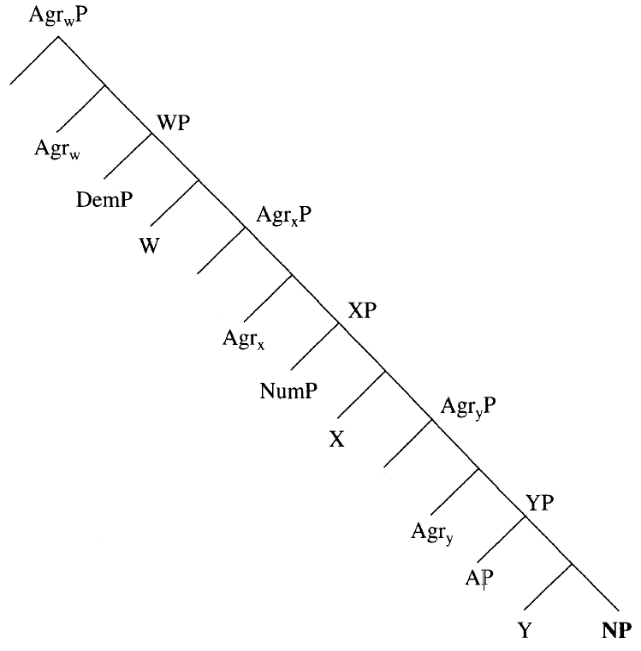
\includegraphics[width=\textwidth]{figures/baron-img1.png}
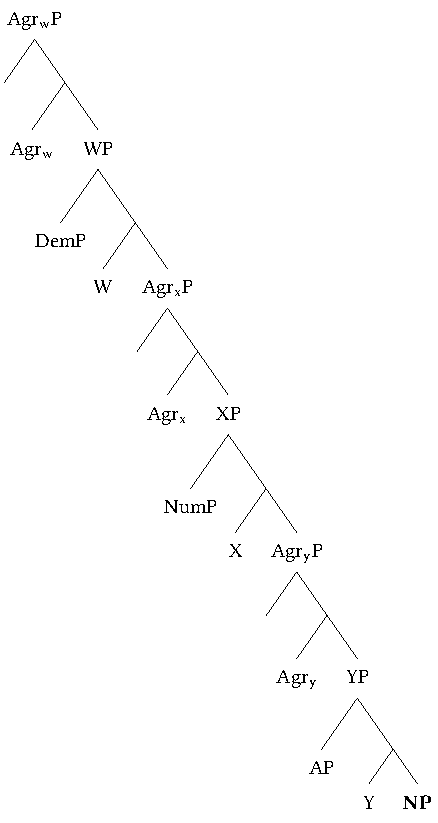
\includegraphics{figures/baron-img1.pdf} % externalised b/c of awkward PGF bug.
\caption{the cartographic representation of DPs (adapted from \citealt[(2)]{Cinque2005}).} 
\label{fig:baron:1}
\end{figure}

Note here that, in Cinque’s account, Num, Dem, and A are heads of their own functional projections (henceforth FPs) above NP. Those FPs merge in the Specifier of phrases (here WP, XP, and YP) that are all sisters to an Agree node, head of an AgrP where NP potentially lands when undergoing movement. From a Minimalist perspective \citep{Chomsky1995}, such a structure violates the economy principle by assuming that additional and potentially unnecessary elements merge into the syntactic structure. Therefore, and in an effort to preserve Cinque’s hierarchy, I assume the syntactic structure in \REF{ex:baron:2} below, where functional elements all merge directly above NP and below D as heads of their own projections, and where AgrPs are eliminated.\footnote{The present analysis for the surface DP word order in Nafara does not justify the need for AgrPs to be generated in the syntax.} Adjectives are not included in \REF{ex:baron:2}. Their location and behavior will be discussed more thoroughly in \sectref{sec:baron:2.1.5}.


\ea{} \label{ex:baron:2}
 [\textsubscript{DP} … D [\textsubscript{DemP} … Dem [\textsubscript{NumP} … Num [\textsubscript{NP} … N ]]]]
\z

The remainder of \sectref{sec:baron:2.1} will focus on the distribution and properties characteristic of each functional and lexical category represented in Nafara DPs. 


\subsubsection{Determiners}
\label{sec:baron:2.1.2}
Nafara determiners agree in gender and number with the noun they determine. They obligatorily attach to the right edge of the noun in simple DPs, as in \REF{ex:baron:3}. However, in the presence of AP, they attach to the AP final element, as in \REF{ex:baron:4}. It is important to note here the variable placement of the adverb in the AP.


\ea\label{ex:baron:3}
  \ea[]{
  \gll lo  \textbf{-gəl}\\
    mango \textbf{-}\textbf{\textsc{def.3.pl}}\\
  \glt \textit{‘the} \textit{mangoes’}}
 \ex[*]{
 \gll \textbf{gəl}    lo          \\
   \textbf{\textsc{def.3.pl}}   mango \\ 
  \glt \textit{‘the} \textit{mangoes’}}
\z
\z

\ea\label{ex:baron:4}
\gll   lo [(dɛl) tã     / tã   (tɛl) ]  -gəl \\
   mango [(very) sweet / sweet (very) ] -\textsc{def.3.pl}\\
 \glt  ‘the very sweet mangoes’  
\z

\citet{Cinque2005} does not account for determiners and how or where they surface in the DP. Because they are separate morphemes in Nafara, and because it is the only DP-internal element encoding definiteness, I take the definite marker to be the realization of the D head, merging as the sister to the highest DP-internal functional projection, as in \REF{ex:baron:2} above. That D head is spelled out \textit{in} \textit{situ}, cliticizing to the final extended noun phrase element located in its specifier, as shown in \sectref{sec:baron:2.2}.


\subsubsection{Demonstratives}
\label{sec:baron:2.1.3}
Demonstratives also inflect for number and gender. They necessarily follow the determiner, as shown in \REF{ex:baron:5}.

\ea\label{ex:baron:5}
\ea[]
  {\gll  pɔm    tã   -bɛl    \textbf{bal}  \\
  apple    sweet  -\textsc{def.1.pl}    \textbf{\textsc{dem.1.pl}}    \\
\glt  \textit{‘these} \textit{sweet} \textit{apples’}}

\ex[*]
{\gll pɔm    \textbf{bal}   tã     -bɛl\\
  apple    \textbf{\textsc{dem.1.pl}}     sweet  \textsc{-def.1.pl}  \\
\glt  \textit{‘these} \textit{sweet} \textit{apples’}}
\z
\z

Following \citegen{Cinque2005} account, I assume that they merge rather high in DP, as the head of a functional projection DemP. 


\subsubsection{Numerals}
\label{sec:baron:2.1.4}
As shown below, numerals occur in DP-final position. Because the literature on numerals has not led to any consensus on their syntax, both cross-linguistically and within languages, and due to the fact that I have no further evidence to motivate a more elaborate account for the distribution and properties of numerals in Nafara, I follow \citet{Cinque2005} in assuming that they merge as the head of a functional projection NumP.\footnote{Cross-linguistically, numerals have either been analyzed as lexical or functional categories, showing great cross-linguistic differences (\citealt{Danon2012,Ionin2006}, among others).} 


\ea\label{ex:baron:6}
\glt {‘one’} 
\ea
\gll pɔm   -u   \textbf{nuã} \\
apple -\textsc{def.1.sg}   \textbf{one.\textsc{1}}   \\
\glt \textit{‘the} \textit{one} \textit{apple’}
\ex
\gll ʧi   -g   \textbf{nuŋgɔ}   \\
tree -\textsc{def.2.sg}    \textbf{one.\textsc{2}}     \\
\glt \textit{‘the} \textit{one} \textit{tree’}
\ex
\gll lo   -n   \textbf{nunã}\\
mango -\textsc{def.3.sg}    \textbf{one.\textsc{3}}\\
\glt \textit{‘the} \textit{one} \textit{mango’}    
\z
\z

\ea\label{ex:baron:7}
\glt {‘seven’}
\ea
\gll pɔm -u \textbf{kɔrʃi}   \\
apple -\textsc{def.1.pl} \textbf{seven}     \\
\glt \textit{‘the} \textit{seven} \textit{apples’}
\ex
\gll ʧi -i \textbf{kɔrʃi}           \\
tree -\textsc{def.2.pl} \textbf{seven}  \\
\glt \textit{‘the} \textit{seven} \textit{trees’}
\ex
\gll lo -gel \textbf{kɔrʃi}\\
mango -\textsc{def.3.pl} \textbf{seven}\\
\glt \textit{‘t}\textit{he} \textit{seven} \textit{mangoes’}
\z
\z

Note here that while ‘seven’ in \REF{ex:baron:7} – as well as any other number in the language – does not inflect for gender, the number ‘one’ in \REF{ex:baron:6} along with all numbers compounded with ‘one’ do. For this reason, I argue that ‘one’ merges in Num with an unvalued gender feature [u\textsc{gen}]. Following both \citet{Greenberg1963} and \citet{Cinque2005}, I assume NumP to be below DemP in the functional projection hierarchy. The DP word order in Nafara is [N A D Dem Num] as in \REF{ex:baron:1}, repeated in \REF{ex:baron:8} below.

 
\ea\label{ex:baron:8}
\glll lo  tã -gəl  gal  kɔrʃi\\
mango sweet -\textsc{def.3.pl} \textsc{dem.3.pl} seven\\
N  Adj  -D  Dem  Num\\
\glt \textit{‘these} \textit{seven} \textit{sweet} \textit{mangoes’}
\z


\subsubsection{Adjectives}
\label{sec:baron:2.1.5}
So far, I have argued that attributive adjectives directly follow the noun they modify, as in \REF{ex:baron:9a} below. The ungrammaticality of \REF{ex:baron:9b} and \REF{ex:baron:9c} shows that attributive adjectives that occur in postnominal position (that is to say most adjectives in the language) cannot occur in prenominal position.
 
\ea\label{ex:baron:9}
\ea[]
{\gll lo    \textbf{tã}          -gəl         \label{ex:baron:9a} \\
mango  \textbf{sweet}     -\textsc{def.3.pl}    \\
\glt     \textit{‘the} \textit{sweet} \textit{mangoes’}}        
 
\ex[*]
{\gll \textbf{tã}    lo    -gəl         \label{ex:baron:9b}    \\
\textbf{sweet}    mango  -\textsc{def.3.pl}    \\
\glt     \textit{‘the} \textit{sweet} \textit{mangoes’} }

\ex[*]
{\gll \textbf{tã}          -gəl     lo   \label{ex:baron:9c} \\
    \textbf{sweet}    -\textsc{def.3.pl}  mango    \\
\glt      \textit{‘the} \textit{sweet} \textit{mangoes’}  }
\z
\z

There are however certain adjectives that can only occur prenominally. It is the case for adjectives of nationality, as shown in \REF{ex:baron:10a}.


\ea\label{ex:baron:10}
\ea[]
{\gll \textbf{kodivware}     ʃju  -u   \label{ex:baron:10a} \\
   \textbf{Ivorian}    man   \textsc{-def.3.sg}\\
\glt   \textit{‘the} \textit{Ivorian} \textit{man’}}        

\ex[*]   
{\gll ʃju    -u       \textbf{kodivware} \label{ex:baron:10b} \\
   man    \textsc{-def.1.sg} \textbf{Ivorian}\\
\glt {‘the} \textit{Ivorian} \textit{man’} }
 
\ex[*]
{\gll ʃju    \textbf{kodivware}     -u  \label{ex:baron:10c}\\
     man     \textbf{Ivorian}    -\textsc{def.1.sg}\\
\glt {‘the} \textit{Ivorian} \textit{man’}}    
 
\ex[*]
{\gll \textbf{kodivware}   -u      ʃju   \label{ex:baron:10d}\\
  \textbf{Ivorian}  -\textsc{def.1.sg}    man   \\
\glt {‘the} \textit{Ivorian} \textit{man’} } 
\z
\z


In \REF{ex:baron:10b} and \REF{ex:baron:10c}, we see that the same adjective cannot occur after the noun, either preceding or following the determiner. This does not result in a semantic alteration of the DP, but in complete ungrammaticality. \REF{ex:baron:10d} shows that such adjectives cannot be the host for the determiner clitic. 

\citet{Cinque1994} argues that adjective phrases merge in the Specifier position of functional projections occurring in a fixed order above NP based on a strict hierarchy, as in \REF{ex:baron:11}.


\ea\label{ex:baron:11}
[\textsubscript{FP}  AP  F  [  AP  F  [  AP  F  [\textsubscript{NP}  N  ] ] ] ]
\z

The data above is somewhat surprising, as it contradicts the semantic hierarchy for adjectives proposed by \citet{Cinque1994} according to which adjectives of nationality merge lower than adjectives of quality \citep[96]{Cinque1994}. One major difference here is that Nafara postnominal adjectives are ordered freely, as in \REF{ex:baron:12} below. Therefore, as is, the data does not allow us to posit any specific ranking of adjectives of nationality relatively to other types of adjectives.


\ea\label{ex:baron:12}
\ea
\gll pɔm     tã   ʧɛ     ɲe    -bɛl    \\
apple    sweet   good    red    -\textsc{def.1.pl}\\
\glt {‘the} \textit{sweet} \textit{good} \textit{red} \textit{apples’}



\ex
\gll   pɔm     ʧɛ   tã     ɲe    -bɛl   \\
apple    good  sweet     red    -\textsc{def.1.pl}\\
\glt {‘the} \textit{sweet} \textit{good} \textit{red} \textit{apples’}



\ex
\gll   pɔm     ʧɛ   ɲe    tã     -bɛl    \\
apple    good  red    sweet     -\textsc{def.1.pl}\\
\glt {‘the} \textit{sweet} \textit{good} \textit{red} \textit{apples’}



\ex
\gll   pɔm     ɲe  tã     ʧɛ     -bɛl     \\
apple    red  sweet     good    -\textsc{def.1.pl}\\
\glt {‘the} \textit{sweet} \textit{good} \textit{red} \textit{apples’}
\z
\z

Due to the fact that both pre- and postnominal adjectives exist in Nafara, and because postnominal adjectives can be ordered freely, I follow \citet{Cinque2010} in differentiating between two types of adjectives merging in two distinct positions in the syntax. While postnominal (low) adjectives merge as adjuncts inside NP (which explains their free ordering), prenominal (high) adjectives merge higher in the structure. Following Cinque, the latter are in fact reduced relative clauses (henceforth RC) merging in the Specifier of a projection above NP.

Applying this analysis to Nafara, I propose the syntactic representation in \REF{ex:baron:13} below, where the few semantically selected reduced RC adjectives in the language merge in the specifier of the extended nominal domain that I call ƩP following \citet{Aboh2004}.\footnote{In his account for Gungbe – and ultimately for Gbe languages, \citet{Aboh2004} argues in favor of an extended noun phrase that he calls ƩP. In Gbe (also Niger-Congo), ƩP constitutes the inflectional nominal domain, and ƩP alone undergoes movement up the DP spine for agreement purposes, landing in Spec,DP. While ƩP in Nafara does not apparently constitute a particular inflectional domain, I posit its existence in the language as the extended noun phrase once the higher adjectives have merged.}

%KS This bracketing is wrapping onto a new line and it looks ugly. I need to find a way to fix this
\ea\label{ex:baron:13}
[\textsubscript{DP} … D [\textsubscript{DemP} … Dem [\textsubscript{NumP} … Num [\textsubscript{ƩP} [A\textsubscript{high}P] ${\sum}$ [\textsubscript{NP} … [\textsubscript{NP} N] [A\textsubscript{low}P]]]]]]
\z

Considering the word order [ A\textsubscript{high}  N  A\textsubscript{low}  D  Dem  Num ] in \REF{ex:baron:14}, I argue that high and low adjectives all remain in situ within ƩP during the entire derivation.\footnote{Further data regarding complements to N is called for. The question is left aside and will be the object of future research.}  


\ea\label{ex:baron:14}
\glll kodivware lo ʧɛ tã -gəl gal kɔrʃi\\
   Ivorian mango good sweet  -\textsc{def.3.pl} \textsc{dem.3.pl} seven\\
   A\textsubscript{high}   N  A\textsubscript{low}  A\textsubscript{low}  -D  Dem  Num\\
\glt {‘these} \textit{seven} \textit{good} \textit{sweet} \textit{Ivorian} \textit{mangoes’}
\z

In the following section, I show that only ƩP moves up the DP spine, generating the surface word order. I will illustrate this derivation, and motivate it in \sectref{sec:baron:3}.

 
\subsection{Underlying structure and derivation} 
\label{sec:baron:2.2}
In his DP typology, \citet{Cinque2005} argues that all attested word orders are the result of NP undergoing some type or combination of movements. According to him, total roll-up movement (also referred to as Spec-to-Spec movement with pied-piping) is the least marked type of movement available. Regarding the word order [ N A Dem Num ] (which is the one we observe here in Nafara DPs), Cinque argues that it is rather rare, but derived as in \REF{ex:baron:15}.

%Not sure that this should be in a linguistic example even though this is how the author did it. I think this should just be a block quote
\ea\label{ex:baron:15}
\textbf{(N} \textbf{A} \textbf{Dem} \textbf{Num[eral])} has a derivation in which NP raises past A, followed by pied-piping of the \textit{whose} \textit{picture} type past Num[eral], followed by raising of [N A] without  pied-piping (\textbf{marked}) past Dem.        (\citealt{Cinque2005}: 323(6l))
\z

Cinque argues that what makes this word order rather uncommon is that it is somewhat marked. NP undergoes a combination of roll-up and Spec-to-Spec movement, as shown in \figref{fig:baron:2}, adapted from \citet{Cinque2005}.

  
\begin{figure}
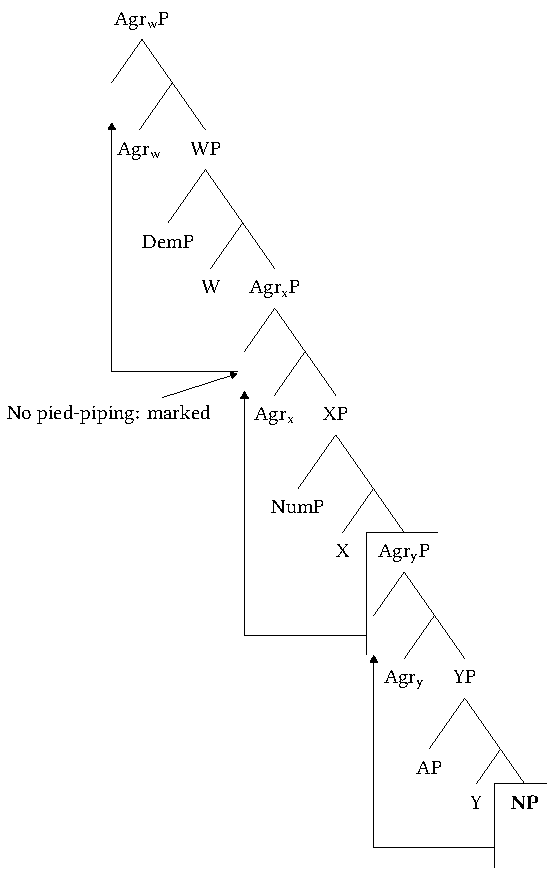
\includegraphics{figures/baron-img2.pdf}
\todo[inline]{Please check tree}
\caption{syntactic derivation for the word order N A Dem Num (adapted from \citealt{Cinque2005}).} 
\label{fig:baron:2}
\end{figure}

In \sectref{sec:baron:2.1.5}, I have established that low adjectives are adjuncts inside NP, and high adjectives merge in Spec,ƩP, an extended nominal projection. Therefore, NP no longer needs to raise past AP and then raise along with AP past Num. Instead, the entire ƩP, including the high and low attributive adjectives, moves up. \figref{fig:baron:3} is a tree representation of the phrase in \REF{ex:baron:16} where this movement is illustrated.


\ea\label{ex:baron:16}
kodivware lo dɛl tã -gəl gal kɔrʃi\\
   Ivorian mango very  sweet  -\textsc{def.3.pl} \textsc{dem.3.pl} seven  \\
\glt {‘these} \textit{seven} \textit{very} \textit{sweet} \textit{Ivorian} \textit{mangoes’}
\z

\begin{figure}
%%[Warning: Draw object ignored]
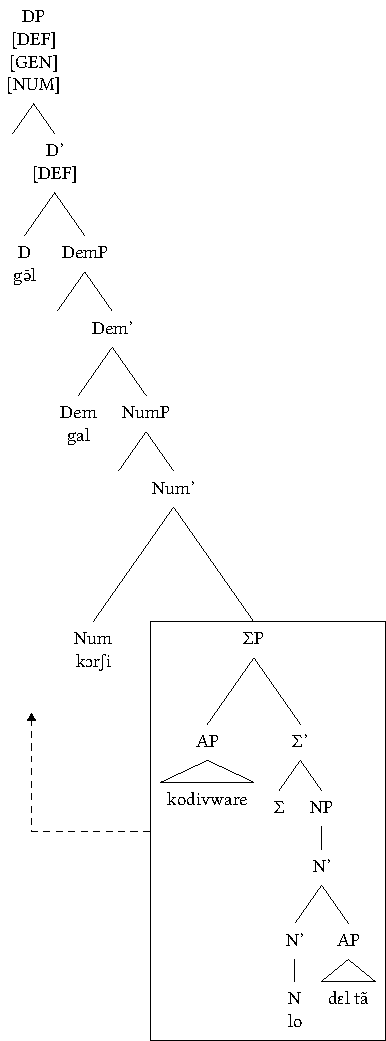
\includegraphics{figures/baron-img3.pdf}
\caption{Feature Percolation in Nafara DPs.\todo[inline]{Please check tree}}
\label{fig:baron:3}
\end{figure}

The syntactic structure in \figref{fig:baron:3} clearly shows that, to obtain the desired word order [ A\textsubscript{high} N A\textsubscript{low} D Dem Num ], ƩP must move up without pied-piping and eventually reach Spec,DP (to precede D, Dem, and Num in that order). Therefore, and contra Cinque in \REF{ex:baron:15} and \figref{fig:baron:2}, I argue that ƩP undergoes a uniform Spec-to-Spec movement without pied-piping all the way up. However, this movement must be correctly motivated. 

In \sectref{sec:baron:2.3}, I demonstrate that movement is triggered by syntactic agreement with N. Due to some agreement effects that I will explain, ƩP is the phrase that gets selected, and raises to Spec,DP by way of Spec-to-Spec movement.
 
\subsection{Agree and DP word order}
\label{sec:baron:2.3}
\subsubsection{Agree}

As previously mentioned, number and gender are active features of Nafara nominal concord. The phrase in \REF{ex:baron:1}, repeated here in \REF{ex:baron:17}, shows that both the determiner and the demonstrative agree in number and gender. 


\ea\label{ex:baron:17}
lo tã -gəl gal kɔrʃi\\
   mango sweet -\textsc{def.3.pl} \textsc{dem.3.pl} seven\\
\glt {‘these} \textit{seven} \textit{sweet} \textit{mangoes’}
\z

Debatably, nominal concord has been argued to be the result of an operation called Agree (\citealt{Chomsky2000,Chomsky2001}, also considered responsible for subject-verb agreement (\citealt{Baker2008,Carstens2001,Collins2004}, among others). One version of the operation is provided in \REF{ex:baron:18}.


\begin{exe}\ex\label{ex:baron:18}
\textbf{Agree} \citep[(26)]{Norris2014}\\
A probe X establishes an Agree relation with a goal YP, where:
\xlista
\ex X c-commands YP,
\ex X lacks values for uninterpretable features that can be supplied by the values of  matching features on Y, 
\ex Y lacks values for uninterpretable features that can be supplied by X, 
\ex No potential goal intervenes between X and Y, 
\ex X and Y are in the same phase.
\endxlista
Agree supplies the values of each category’s uninterpretable features from matching features of the other category, with the two features coalescing into a single shared feature.
\end{exe}


Let us now see how this operation can account for DP-internal agreement and word order in Nafara.


\subsubsection{Agree, EPP, and ƩP movement}

I argue here that D merges with a set of features that contains at least one valued feature – definiteness [\textsc{def}], and two unvalued features – number [{\NUM}] and gender [{\GEN}]. Additionally, D merges with an EPP feature. Similarly, Dem merges with unvalued [{\NUM}] and [{\GEN}] features, and the numeral arguably merges as the head of NumP with a gender feature that is unvalued (that is at least the case for ‘one’, overtly inflecting for gender as shown in \REF{ex:baron:6}).  

By way of Agree, all these functional elements look down their c-command domain for the missing values. As N comes from the lexicon with both [{\NUM}] and [{\GEN}], it is the best possible goal for all of them to probe down to. 

While N is the best potential goal, it is ƩP that moves up. In fact, the same Agree relation through which DP-internal functional elements probe down to N selects ƩP to move up to Spec,DP. In his account for Estonian concord, \citet{Norris2014} argues that the DP-internal agreement pattern observed in the language is made possible by a syntactic principle called Feature Percolation, presented here in \REF{ex:baron:19}.


\begin{exe}\ex\label{ex:baron:19}
\textbf{Feature Percolation} \citep[135 (242)]{Norris2014}
\xlista
\ex All projections of a head X\textsuperscript{0} have the feature-value pairs that X\textsuperscript{0} has.
\ex Let [F:val] be a valued feature on XP.\\
   Let Z\textsuperscript{0} be a head lacking the feature [F].\\
   Let X\textsuperscript{0} and Z\textsuperscript{0} be members of the same extended projection (i.e., both [+N]).\\
   When Z\textsuperscript{0} merges with XP, projecting ZP, ZP also has the valued feature [F:val].
\endxlista
\end{exe}


According to \REF{ex:baron:19}, as heads merge into the structure with valued features, those same features percolate to the phrase those heads project. In \figref{fig:baron:4}, I show how this principle applies in the Nafara DP. By way of Feature Percolation, and due to the fact that ƩP is nominal, I argue that the features \textsc{[gen]} and \textsc{[num]} percolate all the way up to ƩP. 

Since agreement with N occurs all the way up the DP spine, I argue that ƩP undergoes Spec-to-Spec movement up to Spec,DP where the EPP feature on D is satisfied.

  
\begin{figure}
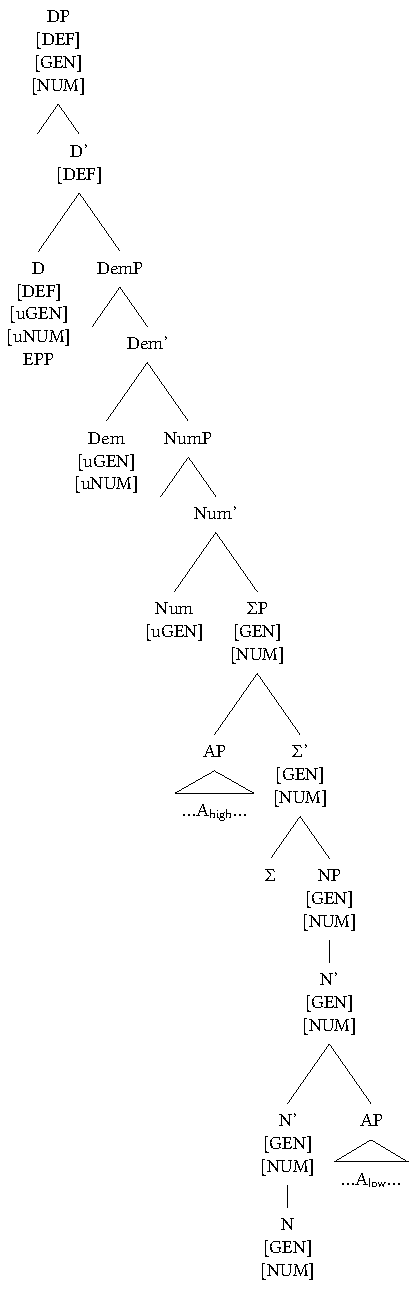
\includegraphics[height=\textheight]{figures/baron-img4.pdf}
\caption{Feature Percolation in Nafara DPs0\todo[inline]{Please check tree}.}
\label{fig:baron:4}
\end{figure}


\section{Conclusions}
\label{sec:baron:3}
%%[Warning: Draw object ignored]
%%[Warning: Draw object ignored]
%%[Warning: Draw object ignored]
In this paper, I have accounted for the structure and word order occurring in Nafara DPs. Following \citet{Cinque2005}, I argue for D > Dem > Num > A > N to be the DP-internal hierarchy. Additionally, and following \citet{Cinque2010}, I argue that there are two distinct types of attributive adjectives, that I refer to as high and low, and that do not seem to be interchangeable in the language. Finally, I argue that the surface word order is derived by moving ƩP to Spec,DP, for agreement purposes and due to the presence of an EPP feature on D. Because it is structurally higher than ƩP, Num does not undergo movement. For this reason, it surfaces in DP final position. The Spec-to-Spec movement of ƩP is illustrated in \REF{ex:baron:20} below.

\ea\label{ex:baron:20}\small
% % 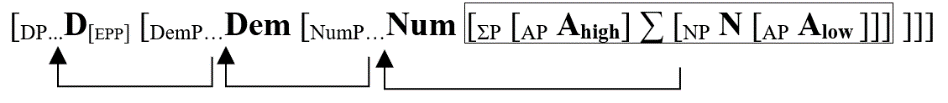
\includegraphics[width=\textwidth]{figures/baron-img5.png}
[\textsubscript{DP\ConnectTail{...}}\textbf{D}\textsubscript{[EPP]} [\textsubscript{DemP\ConnectHead*[2ex]{\ConnectTail{...}}}\textbf{Dem} [\textsubscript{NumP\ConnectHead*[2ex]{\ConnectTail{...}}}\textbf{Num} \ConnectHead*[2ex]{\tikz[baseline]\node[draw,anchor=base,inner ysep=1ex]{[\textsubscript{ΣP} [\textsubscript{AP} \textbf{A}\textsubscript{\textbf{high}}] Σ [\textsubscript{NP} N [\textsubscript{AP} \textbf{A}\textsubscript{\textbf{low}}]]]};}]]
\z
  


%%These bib entries are also in localbibliography.bib

%Bendor-Samuel, John. 1971. Niger–Congo: Gur. In: Thomas Sebeok & Jack Berry (eds.), Linguistics in sub-saharan Africa (Current trends in linguistics 7). The Hauge/Paris: Mouton. 141–178.Bendor-Samuel 1971

%Cinque, Guglielmo. 1994. On the evidence for partial N movement in the Romance DP. In Paths toward Universal Grammar, ed. by Guglielmo Cinque, Jan Koster, Jean- Yves Pollock, Luigi Rizzi, and Raffaella Zanuttini, 85-110. Washington, DC: Georgetown University Press.


%Collins, Chris. 2004. The agreement parameter. In Anne Breitbarth and Henk van Riemsdijk, eds. Triggers. 115-136. New York: Mouton.


 

%Manessy, Gabriel. 1975. Les langues Oti-Volta. Paris: SELAF.

%Naden, Anthony. 1989. Gur. In John Bendor-Samuel and Rhonda Hartell (eds.), The Niger-Congo languages. A classification and description of Africa’s largest language family. Lanham, New York, London : University Press of America. 140–168.



\section*{Abbreviations}

% % Glossing and abbreviations are as follows: 

\begin{multicols}{3}
\begin{tabbing}
\textsc{indef} \= demonstrative\kill
A(dj) \> adjective\\
1 \> gender1\\
2 \> gender2\\
3 \> gender3\\
D \> determiner\\
\textsc{def} \> definite\\
Dem \> demonstrative\\
\textsc{indef} \> indefinite\\
Num \> numeral\\
\textsc{pl} \> plural\\
SG \> singular
\end{tabbing}
\end{multicols}

% % \section*{Acknowledgements}

{\sloppy
\printbibliography[heading=subbibliography,notkeyword=this] 
}
\end{document}
